\begin{minipage}{0.45\textwidth}
    \[
    \sigma(x) = \frac{1}{1 + e^{-x}}
    \]
\end{minipage}
\hfill
\begin{minipage}{0.45\textwidth}
    \centering
    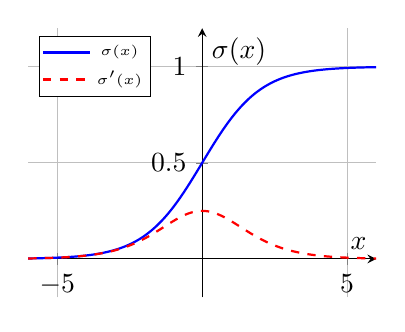
\begin{tikzpicture}[scale=1]
        \begin{axis}[
            xlabel=$x$,
            ylabel=$\sigma(x)$,
            grid=major,
            axis lines=middle,
            xmin=-6, xmax=6,
            ymin=-0.2, ymax=1.2,
            samples=200,
            width=6cm,
            height=5cm,
            legend pos=north west,
            legend style={font=\tiny, inner sep=1pt}
        ]
            \addplot[blue, thick, domain=-6:6] {1/(1+exp(-x))};
            \addlegendentry{$\sigma(x)$}
            \addplot[red, dashed, thick, domain=-6:6] {1/(1+exp(-x)) * (1 - 1/(1+exp(-x)))};
            \addlegendentry{$\sigma'(x)$}
        \end{axis}
    \end{tikzpicture}
\end{minipage}
